
\documentclass[journal]{IEEEtran}

\usepackage{color}
\usepackage{isotope}
\usepackage{graphicx,subfigure}
\usepackage{dcolumn}% Align table columns on decimal point
\usepackage{bm}% bold math
\usepackage[latin9]{inputenc}

\usepackage[pdfborder=000,pdftex=true]{hyperref}
\usepackage{amsmath}
\usepackage{balance}

\begin{document}

\title{Software system for data acquisition and real-time analysis operating the ATLAS-TPX network}

\author{Benedikt~Bergmann, Jakub~Begera, Petr~Burian, Josef~Janecek, Petr~Manek, Stepan~Polansky, Stanislav~Pospisil~\IEEEmembership{Senior~Member,~IEEE}

\thanks{B. Bergmann, J. Begera, P. Burian, J. Janecek, P. Manek, S. Polansky, S. Pospisil are with the Institute of Experimental and Applied Physics, Czech Technical University in Prague, Horska 3a/22, 128 00 Praha 2-Albertov, Czech Republic.

P. Burian is also with the Faculty of Electrical Engineering, University of West Bohemia.\protect\\
The work has been done in the frame of the Medipix collaboration. This research project has been supported by the Ministry of Education, Youth and Sports of the Czech Republic under project numbers: LM2015058 and LG15052\protect\\
E-mail: jakub.begera@cvut.cz, petr.manek@cvut.cz}
}

\markboth{}%
{J. Begera, P. Manek \MakeLowercase{\textit{et al.}}: The ATLAS-TPX detector network}


\maketitle

%\tableofcontents

\begin{abstract} 
TODO
\end{abstract}

\section{\label{sec:introduction}Introduction}
TODO

\section{\label{sec:device}Timepix Detector}
Each ATLAS-TPX device consists of two Timepix~\cite{Llopart2007} readout chips with silicon sensor layers of thicknesses 300\,$\mu$m and 500\,$\mu$m facing each other. They are interlaced by a set of neutron converters. The Timepix ASIC (application specific integrated circuit) divides the sensor area into a square matrix of $256 \times 256$ contiguous pixels with a pixel dimension of 55\,$\mu$m. It allows a configuration of each pixel in either of the three modes of operation: 
\begin{itemize}
\item In the spectroscopic Time-over-Threshold (ToT) mode the energy deposition in the sensor material is measured.
\item In the Time-of-Arrival (ToA) mode the time from an interaction with respect to the end of the exposure is recorded (precision up to 25\,ns).
\item In the counting mode, the number of interactions with energies above 5\,keV during the exposure time are counted.
\end{itemize}

Data are taken in so-called frames, representing the counter contents of all individual pixels after an adjustable exposure time (often also referred to as frame acquisition time). In each frame, interacting quanta of ionizing radiation can be seen as tracks on the pixel matrix, which have characteristic shapes, depending on the particle range in silicon, its deposited energy, angle of incidence, and particle type. 

\section{\label{sec:hardware}Hardware Architecture}
TODO

\begin{figure}[tbp]
	\centering
        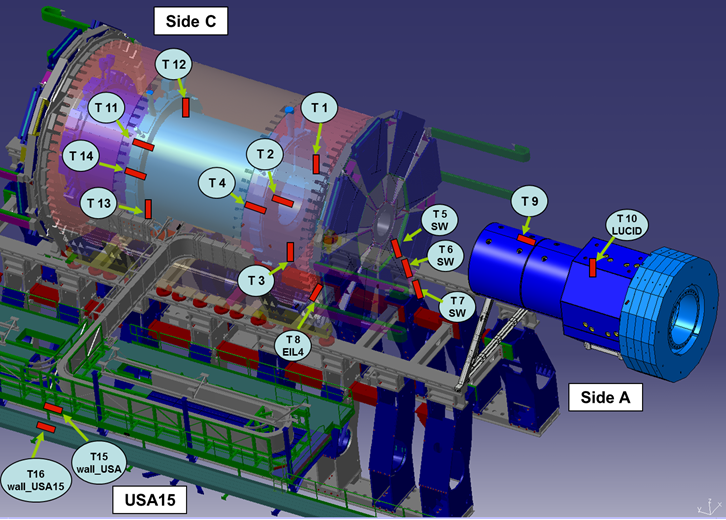
\includegraphics[clip, width=.45\textwidth, angle = 0 ]{Plots/ATLASTPX.png}
      \caption {Artistic view of the device positions of the ATLAS-TPX network in the ATLAS experiment.}
    \label{fig:positions}
\end{figure}

\begin{figure}[tbp]
	\centering
        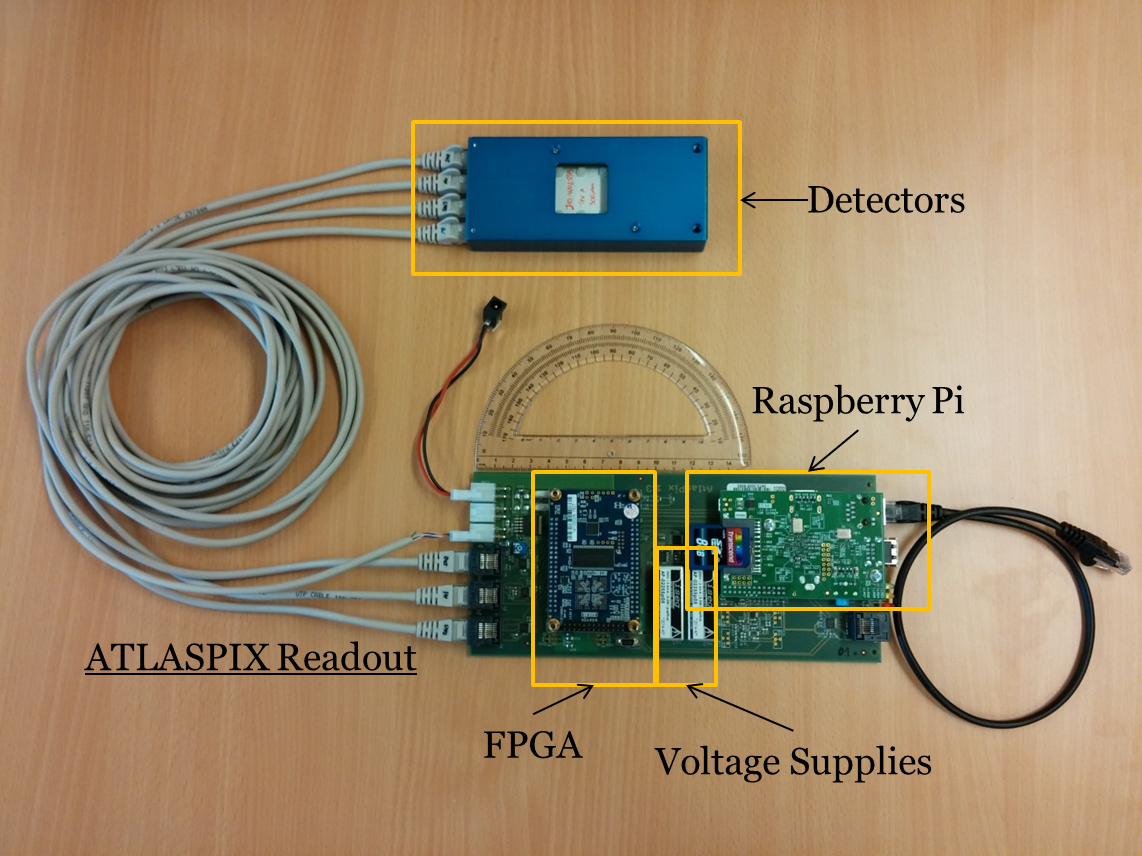
\includegraphics[clip,width=.45\textwidth, angle = 0 ]{Plots/ATLASPIX.png}
      \caption {ATLAS-TPX device, connected to its readout system through three Ethernet cables. The readout system consists of an FPGA, handling the device settings and operation, and a Raspberry Pi minicomputer for sending the data to the control PC in human readable format. Two voltage supplies are used for feeding the proper bias to each of the sensor layers.}
    \label{fig:device_with_readout}
\end{figure}

\begin{figure}[tbp]
	\centering
        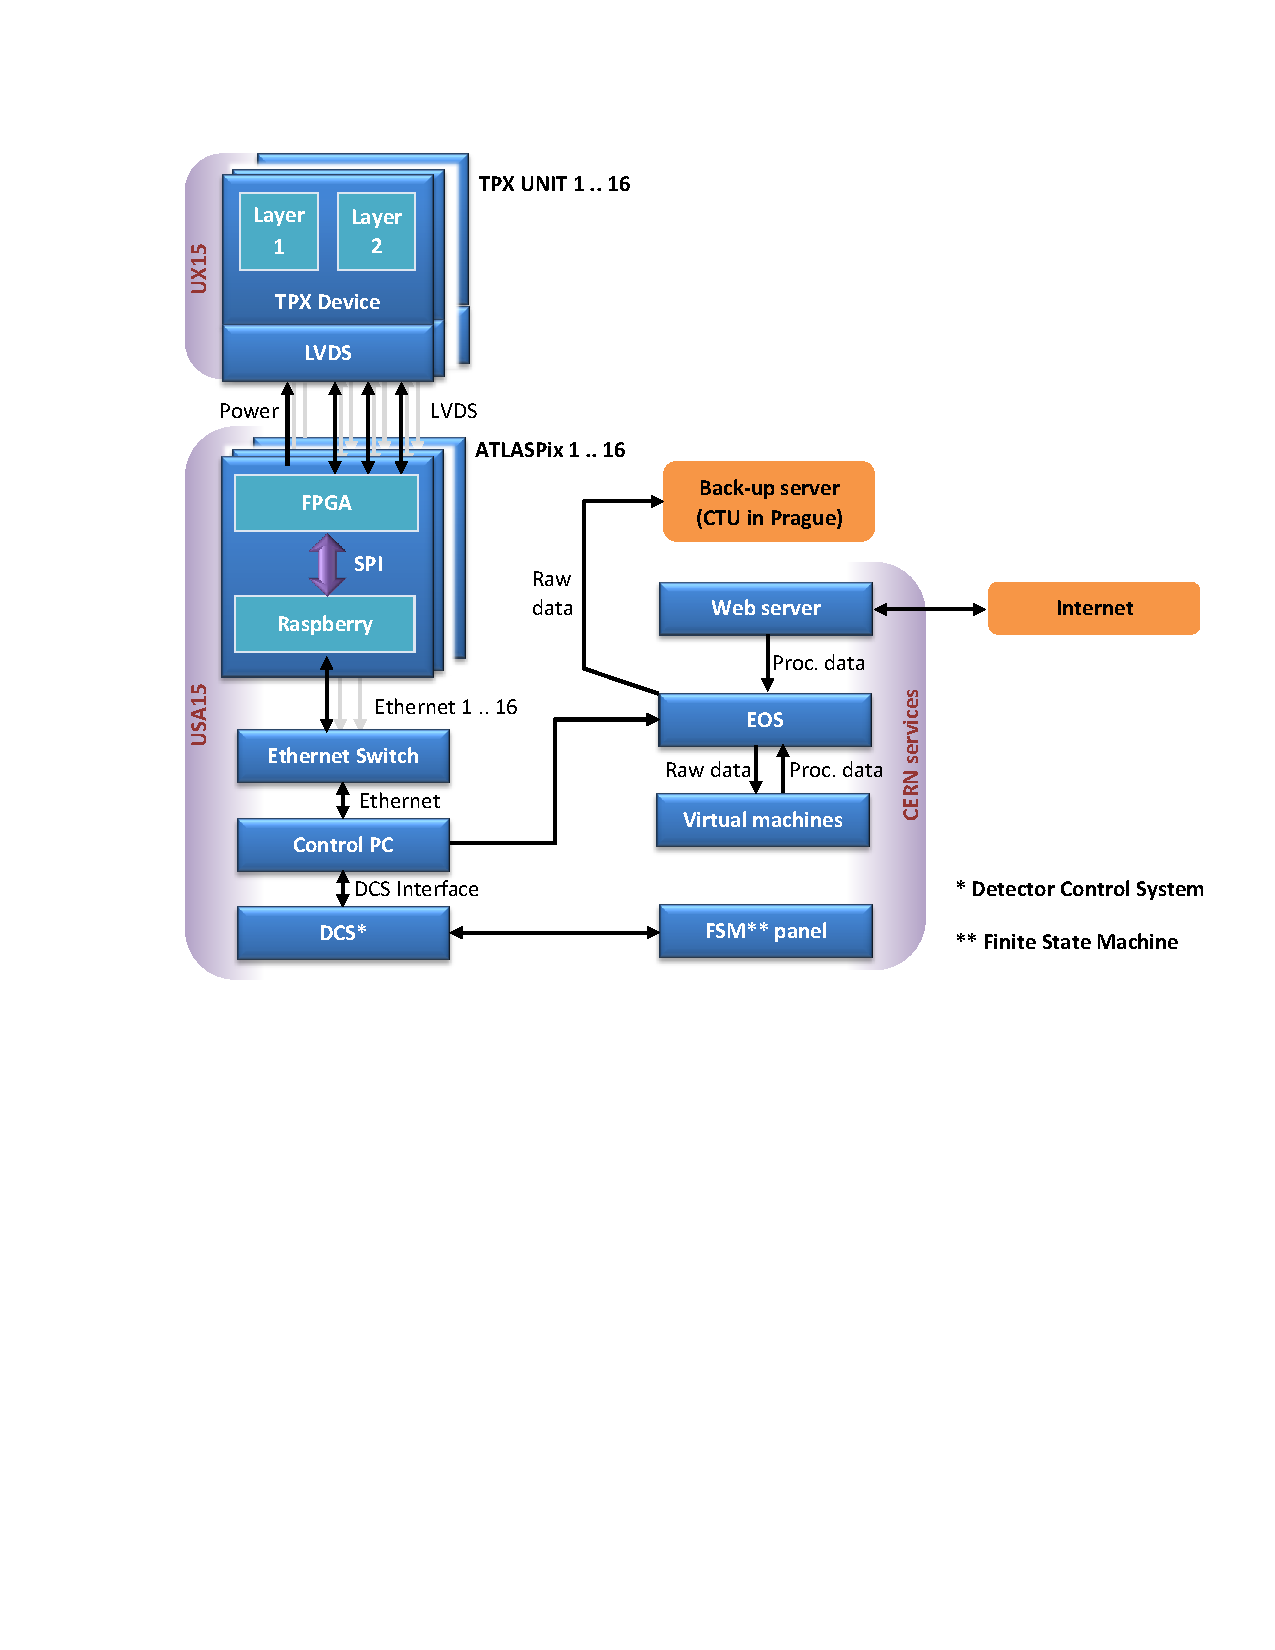
\includegraphics[clip, trim={2cm 11.2cm 0cm 2.6cm}, width=.5\textwidth, angle = 0 ]{Plots/Doc1.pdf}
      \caption {Scheme of the readout, detector control, and data flow.}
    \label{fig:data_flow}
\end{figure}

\section{\label{sec:acquisition}Data Acquisition Software}
TODO

\section{\label{sec:analysis}Data Analysis Software}
TODO

\section{\label{sec:dal}Visualization Application}
TODO

\section{\label{sec:conclusion}Conclusion}
TODO

%
\bibliographystyle{IEEEtran}
\bibliography{ieee2016}% Produces the bibliography via BibTeX.
%\begin{thebibliography}{10}
%\end{thebibliography}
%
\end{document}
%
% ****** End of file apssamp.tex ******
